\label{chapter-5}
In the previous chapter a set of suggestions for improving a BPMN diagram where listed. As it was also mentioned, not all of these improvements can be automated. 

This chapter will provide a example how the mentioned not automatable and automatable suggestions can be applied together to an existing BPMN model. 

At first, the example BPMN model used for this case study and the evaluation that is done by the software on this BPMN will be explained. After that, all suggestions as they are listed in section \ref{last} will be implemented one by one, using the software evaluation as aid. 

In the end, the original BPMN will be compared with the final result using quantitative measures as described in section \ref{quant}.

\section{The example model}
The used BPMN model for this chapter will be a fictitious client registration process which was adapted from a real live process used in the telecommunication sector in order to be used in this thesis. The graphical representation of the process model can be found in figure \ref{fig:example-process} and the full XML structure is in the appendix section \ref{app-1}

\begin{figure}[H]
	\centering
	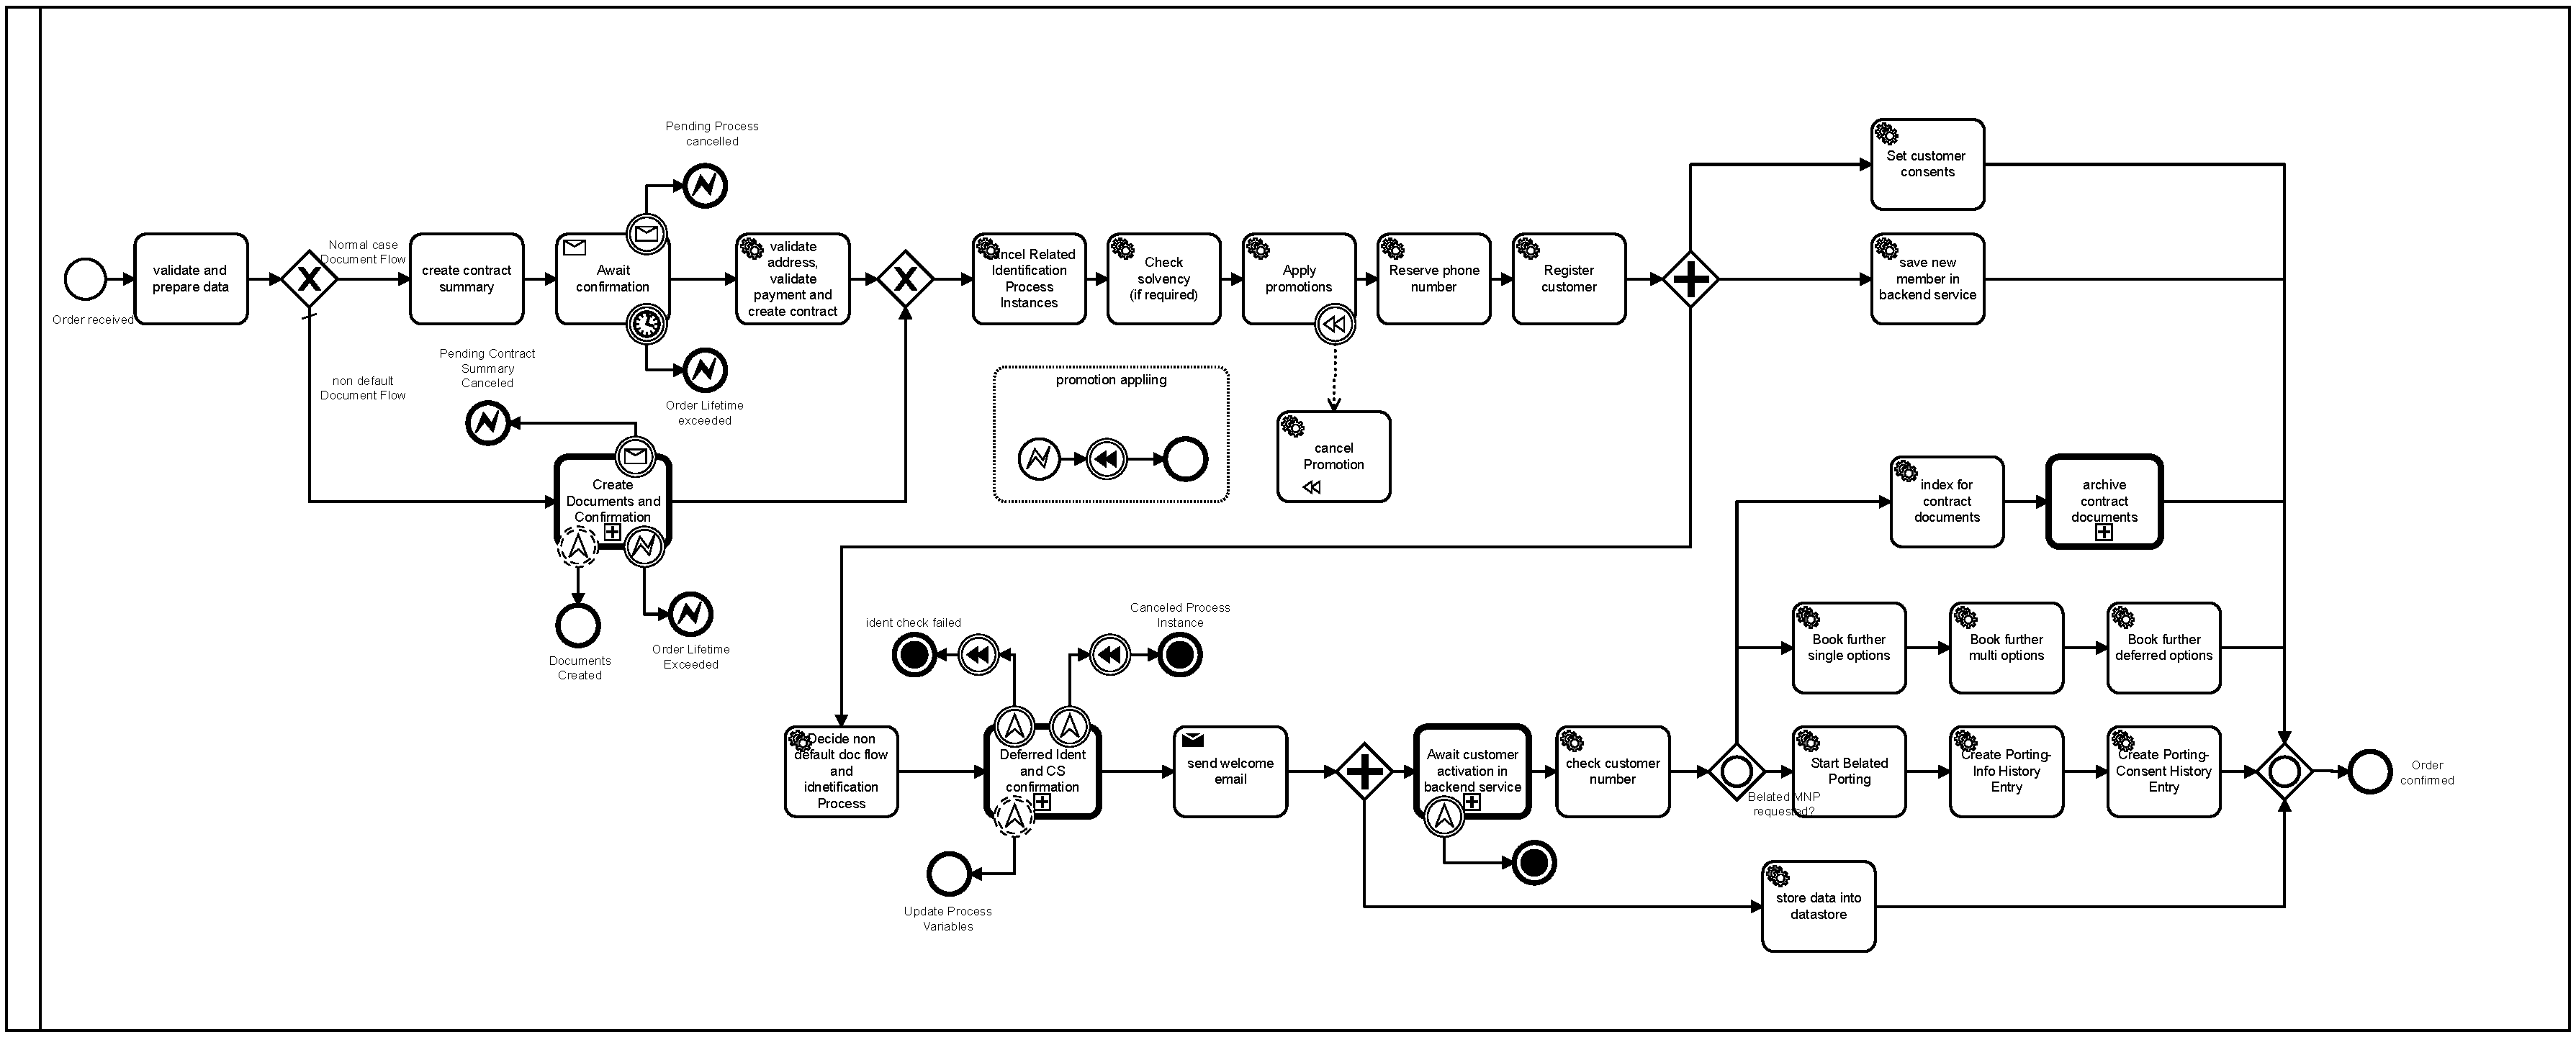
\includegraphics[width=1.7\columnwidth, angle=90 ]{graphics/process-bpmn.pdf}
	\caption{Example of a process where tasks can be merged together} 
	\label{fig:example-process} 
\end{figure}

\section{Evaluation by the Software}
In order to evaluate the best practices that where automated by the software as mentioned in section \ref{last}, the BPMN Model was given as input for the software. The full output can be found in section \ref{app-1} the following output for each Suggestion/Rule was given:
\paragraph{Comply with Naming Conventions}~\\
As described in chapter \ref{naming-con}, this algorithm scans the BPMN model for events, tasks or gateways that have more than five words in their label. The following list of elements is returned that violate this rule:
\begin{lstlisting}[language=json,label=lst:naming]
"effectedElements": [
{
	"id": "ServiceTask_DefaultDocWorkflowPostAwaitConfirmation",
	"name": "validate address, validate payment and create contract",
	"type": "Task"
},
{
	"id": "DecideIdAndCsProcess",
	"name": "Decide non default doc flow and idnetification Process",
	"type": "Task"
},
{
	"id": "save_member_for_riskident",
	"name": "save new member in backend service",
	"type": "Task"
}
\end{lstlisting}


\paragraph{Eliminate Manual Tasks}~\\
When searching for manual tasks in the process (see section \ref{soft-manual}), only one can be identified and is returned:
\begin{lstlisting}[language=json,label=lst:manual]
"effectedElements": [
{
	"id": "data_to_warehouse",
	"name": "store data into datastore",
	"type": "Task"
}
\end{lstlisting}
\paragraph{No two consecutive Tasks handled by the same resource}~\\
Another rule that was implemented was that no two consecutive tasks should be processed by the same resource. The Software identified the following tasks that could be merged with its successor:
\begin{lstlisting}[language=json,label=lst:merge]
"effectedElements": [
{
	"id": "CancelRelatedWebIdent",
	"name": "Cancel Related Identification Process Instances",
	"type": "Task"
},
{
	"id": "ReserveMsisdn",
	"name": "Reserve phone number",
	"type": "Task"
},
{
	"id": "BookAutoTopups",
	"name": "Book further multi options",
	"type": "Task"
},
{
	"id": "ServiceTask_0p0tajd",
	"name": "Start Belated Porting",
	"type": "Task"
},
{
	"id": "ServiceTask_0e2r82f",
	"name": "Create Porting-Info History Entry",
	"type": "Task"
},
{
	"id": "BookSingleTopups",
	"name": "Book further single options",
	"type": "Task"
}
]
\end{lstlisting}
\paragraph{Inclusive Gateways over combining parallel and exclusive Gateways}~\\
As described in section \ref{inc-sw} it is preferred to use inclusive gateways instead of combining parallel and exclusive gateways. The only element that violates that rule in the given BPMN is returned:
\begin{lstlisting}[language=json]
"effectedElements": [
{
	"id": "ParallelGateway_0crudor",
	"name": null,
	"type": "Gateway"
}
]
\end{lstlisting}
\section{Comply with Naming Conventions}
Based on the naming conventions defined in section \ref{naming} unnamed Tasks, Events and Gateways where named and Elements returned in listing \ref{lst:naming} where renamed. In figure \ref{fig:naming-org} a segment of the example BPMN is shown and figure \ref{fig:naming-new} shows the corresponding changes after renaming. 

\begin{figure}[H]
	\centering
	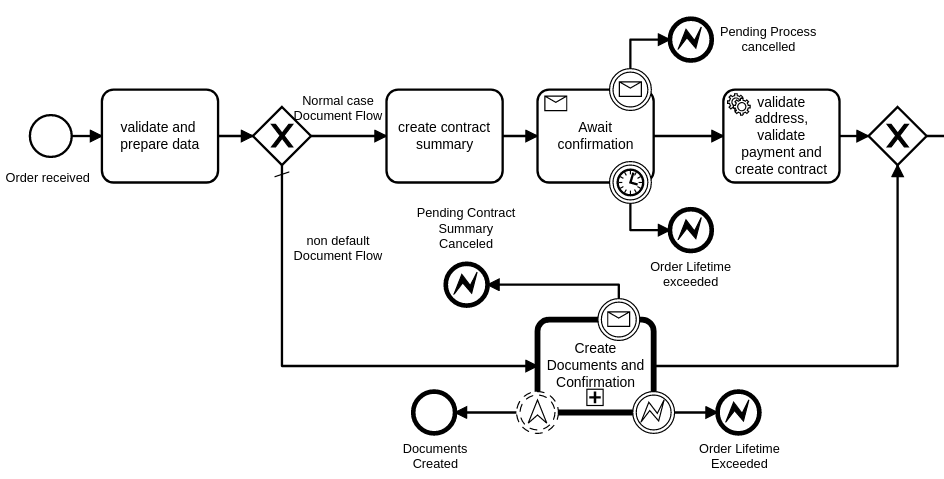
\includegraphics[width=0.9\columnwidth]{graphics/case-study-naming-org}
	\caption{Segment of the BPMN model in figure \ref{fig:example-process}}
	\label{fig:naming-org}
\end{figure}

\begin{figure}[H]
	\centering
	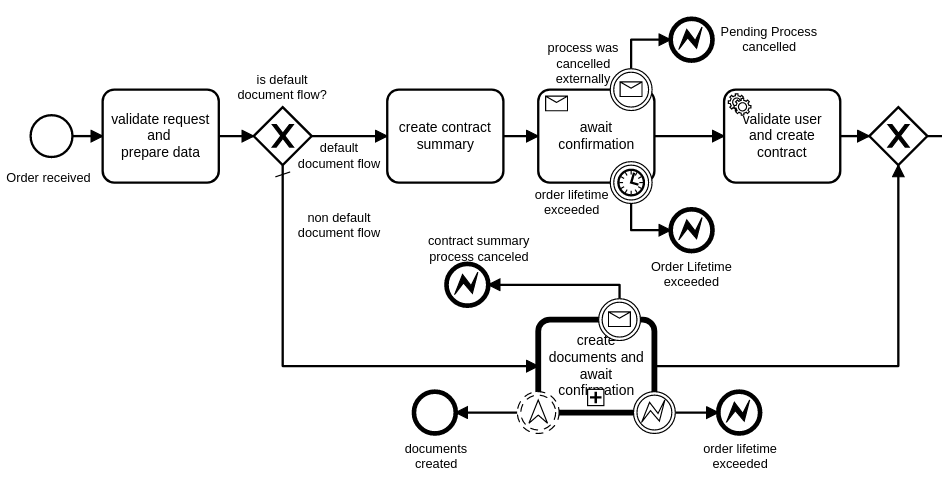
\includegraphics[width=0.9\columnwidth]{graphics/case-study-naming-new}
	\caption{Segment \ref{fig:naming-org} with implementing naming conventions}
	\label{fig:naming-new}
\end{figure}

The full renaming change can be found in the appendix chapter \ref{BPMN-after-naming}. The full XMl representation of this process can be found in \cite{online-BPMN-after-naming}

\section{Eliminate Manual Tasks}
The only manual task in this BPMN model is the \textit{cancel promotion} task. Cancelling promotions can only be done manually by a service agent in this fictitious case and can therefore not be automated. In this case, the manual task can be change into a \textit{user task} and the advantages of a worklist handler can be utilized as described in section \ref{manual}.
The original segment with the manual task can be seen in figure \ref{fig:manual-org}. The corresponding change in this section of the mode is shown in figure \ref{fig:manual-new}. 


\begin{minipage}[t]{0.5\textwidth}
	\begin{figure}[H]
		\centering
		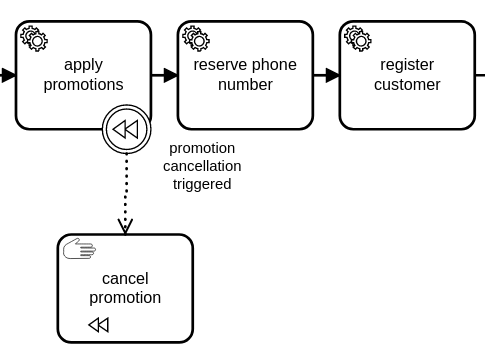
\includegraphics[width=0.8\textwidth]{graphics/case-study-manual-org}
		\caption{Segment of the BPMN model in figure \ref{fig:example-process} with the only manual tasks}
		\label{fig:manual-org}
	\end{figure}
\end{minipage}
\begin{minipage}[t]{0.5\textwidth}
\begin{figure}[H]
	\centering
	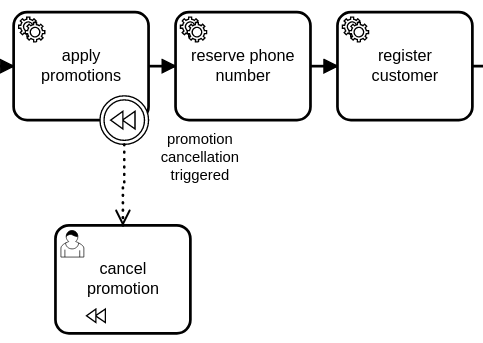
\includegraphics[width=0.8\textwidth]{graphics/case-study-manual-new}
	\caption{Segment that is shown in figure \ref{fig:naming-org} with changing the manual tasks to a user task}
	\label{fig:manual-new}
\end{figure}
\end{minipage}

The full BPMN change can be found in \cite{online-BPMN-after-manual}.

\section{Extend automation boundaries}
Since the process model is already fully automated apart from the \textit{cancel promotion} task and this task is not automatable yet, as already mentioned in the last section, the automation boundaries cannot be extended further. 

\section{No two consecutive Tasks handled by the same resource}
According to the rules described in section \ref{merge-section}, the list of elements given in \ref{lst:merge} can be merged with their direct successor. The segements of the BPMN model with the listed elements can be found in figures \ref{fig:merge-1-org} and \ref{fig:merge-2-org} and the respective change is shown in figures \ref{fig:merge-1-new} and \ref{fig:merge-2-new}. 
\begin{figure}[H]
	\centering
	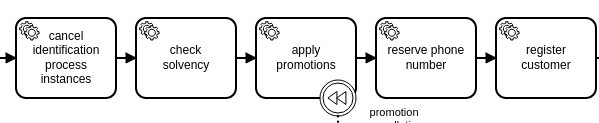
\includegraphics[width=0.8\textwidth]{graphics/case-study-merge-org-1}
	\caption{Segment of the BPMN model in figure \ref{fig:example-process} with consecutive service tasks}
	\label{fig:merge-1-org}
\end{figure}

\begin{figure}[H]
	\centering
	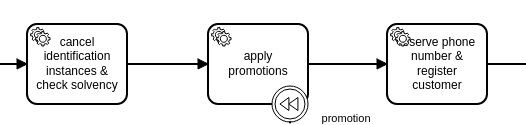
\includegraphics[width=0.8\textwidth]{graphics/case-study-merge-new-1}
	\caption{Segment that is shown in figure \ref{fig:merge-1-org} with merged consecutive service tasks}
	\label{fig:merge-1-new}
\end{figure}

\begin{minipage}[t]{0.5\textwidth}
\begin{figure}[H]
	\centering
	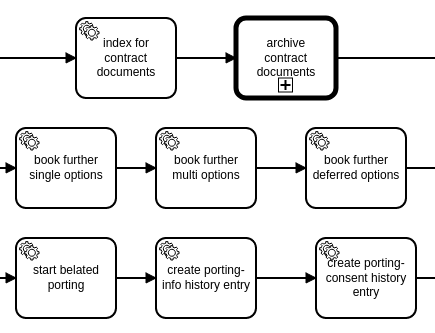
\includegraphics[width=0.95\textwidth]{graphics/case-study-merge-org-2}
	\caption{Segment of the BPMN model in figure \ref{fig:example-process} with consecutive service tasks}
	\label{fig:merge-2-org}
\end{figure}
\end{minipage}
\begin{minipage}[t]{0.5\textwidth}
\begin{figure}[H]
	\centering
	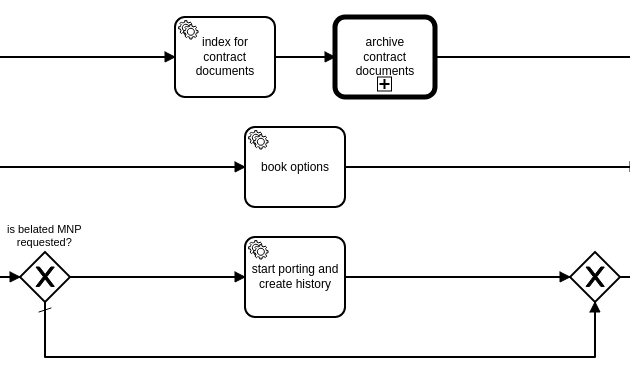
\includegraphics[width=0.95\textwidth]{graphics/case-study-merge-new-2}
	\caption{Segment that is shown in figure \ref{fig:merge-2-org} with merged consecutive service tasks}
	\label{fig:merge-2-new}
\end{figure}
\end{minipage}

The full BPMN change can be seen in the appendix section \ref{online-BPMN-after-merge}. 

\section{Inclusive Gateways over combining parallel and exclusive Gateways}
The only case in this BPMN model where a combination of parallel and exclusive gateways was used instead of an inclusive gateway is in the segment shown in figure \ref{fig:exclusive-org}. The corresponding change in this section of the model is shown in figure \ref{fig:exclusive-new}. 


\begin{figure}[H]
	\centering
	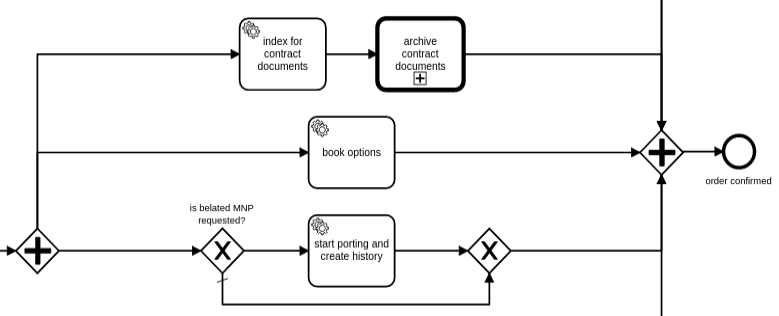
\includegraphics[width=0.8\textwidth]{graphics/case-study-exclusive-org}
	\caption{Segment of the BPMN model in figure \ref{fig:example-process} where parallel and exclusive tasks are combined instead of using an inclusive gateway}
	\label{fig:exclusive-org}
\end{figure}
\begin{figure}[H]
	\centering
	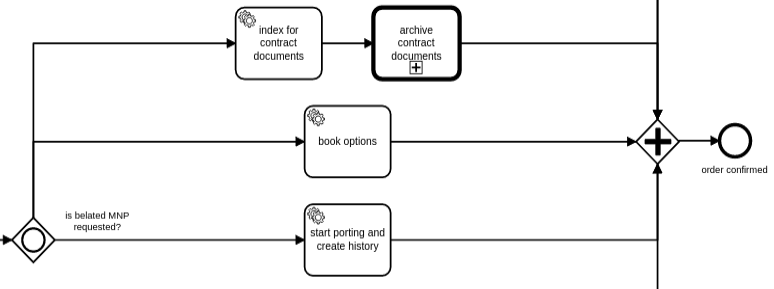
\includegraphics[width=0.8\textwidth]{graphics/case-study-exclusive-new}
	\caption{Segment that is shown in figure \ref{fig:exclusive-org} with using an inclusive gateway}
	\label{fig:exclusive-new}
\end{figure}

The full BPMN change can be found in \cite{online-BPMN-after-exclusive}.

\section{Value Added Analysis}
%TODO

\section{Evaluate Suggestions Quantitative}
%TODO

